\documentclass[mathNotesPreamble]{subfiles}
\begin{document}
\section{JIT 4.2: Lines And Their Equations}
  \begin{defn*}
    The \textbf{slope} of a line is $m=\dfrac{\Delta y}{\Delta x}=\dfrac{y_1-y_2}{x_1-x_2}$. 
    
    The slope is the rate at which $y$ increases or decreases with respect to $x$.
  \end{defn*}
  \begin{defn*}
    The \textbf{point-slope} formula of the line with slope $m$ going through point $(x_0,y_0)$ is 
      $$y-y_0=m(x-x_0)$$
  \end{defn*}
  \begin{ex*}
    Find the equation of the line with slope $m=-3$ that goes through the point $P_1=(2,-5)$. 
    \vfill
  \end{ex*}
  
  \begin{ex*}
    Find the equation of the line that goes through $P_1=(1,-2)$ and $P_2=(-2,3)$.
    \vfill
  \end{ex*}
  
  \pagebreak
  \begin{defn*}
    The \textbf{slope-intercept form} of the line with slope $m$ and intercept $b$ is 
      $$y=mx+b$$
  \end{defn*}
  
  \begin{ex*}
    Find the equation of the line with slope $m=3$ that with intercept $b=-1$. 
    \\[\stretch{0.45}]
  \end{ex*}
  
  \begin{ex*}
    Find the equation of the line that goes through $P_1\!=\!(0,\sfrac12)$ and $P_2\!=\!(4,-\sfrac12)$.
    \vfill
  \end{ex*}
  \pagebreak
  \begin{defn*}
    Two lines, with slopes $m_1$ and $m_2$ are \textbf{parallel} when $m_1=m_2$. 

    Lines are \textbf{perpendicular} when $m_1=-\dfrac{1}{m_2}$
  \end{defn*}
  \begin{ex*}
    Find the line parallel to $f(x)=-\sfrac12x+4$ that goes through the point $P_1=(1,4)$.  Also find the line perpendicular to $f(x)$ that goes through the point $P_2=(2,-3)$.\\[\stretch{1}]
  \end{ex*}
  \begin{ex*}
    (Briggs: 1.2.7) Write a definition of the piecewise linear function $y=f(x)$ that is given in the graph.
    
      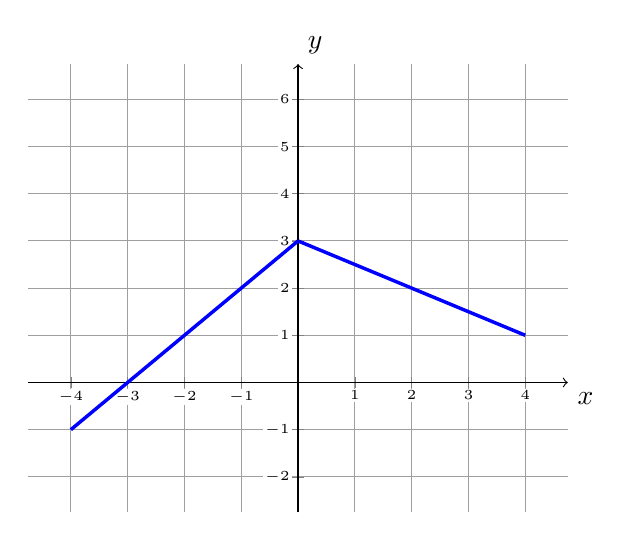
\begin{tikzpicture}[scale=1.0]
        \begin{axis}[
          grid=both,
          grid style={line width=0.35pt, draw=gray!75},
          axis lines=center,
          axis line style={->},
          xmin=-4, xmax=4,
          ymin=-2, ymax=6,
          xtick={-4,-3,...,4},
          ytick={-2,-1,...,6},
          enlargelimits={abs=0.75},
          ticklabel style={font=\tiny,inner sep=0.75pt,fill=white},
          xlabel=$x$, xlabel style={at={(ticklabel* cs:1)},anchor=north west},
          ylabel=$y$, ylabel style={at={(ticklabel* cs:1)},anchor=south west},
          ]
          \addplot[domain=-4:0,blue, line width=1.25pt] {\x+3};
          \addplot[domain=0:4,blue, line width=1.25pt] {-0.5*\x+3};
      \end{axis}
    \end{tikzpicture}\\[\stretch{0.5}]
  \end{ex*}
  \pagebreak
  (Brigs: 1.2.25, 1.2.26) Write a definition of the function whose graph is given.
  \begin{ex*}\ 
  
    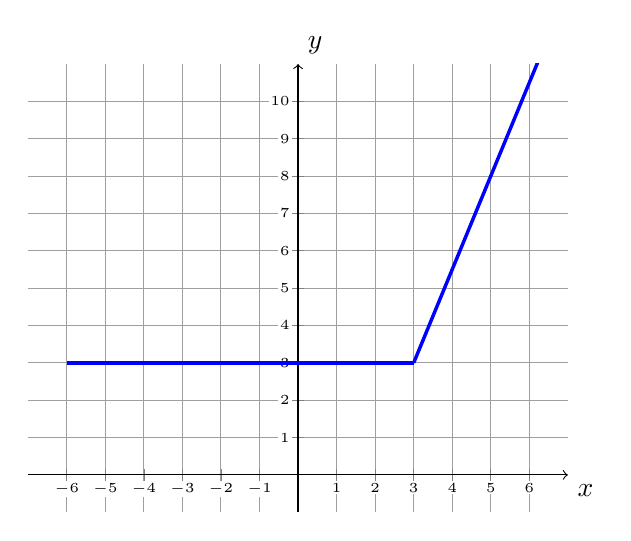
\begin{tikzpicture}[scale=1.0]
        \begin{axis}[
          grid=both,
          grid style={line width=0.35pt, draw=gray!75},
          axis lines=center,
          axis line style={->},
          xmin=-6, xmax=6,
          ymin=0, ymax=10,
          xtick={-6,-5,...,6},
          ytick={0,1,...,10},
          enlargelimits={abs=1.0},
          ticklabel style={font=\tiny,inner sep=0.75pt,fill=white},
          xlabel=$x$, xlabel style={at={(ticklabel* cs:1)},anchor=north west},
          ylabel=$y$, ylabel style={at={(ticklabel* cs:1)},anchor=south west},
          ]
          \addplot[domain=-6:3,blue, line width=1.25pt] {3};
          \addplot[domain=3:7,blue, line width=1.25pt] {5/2*\x-9/2};
      \end{axis}
    \end{tikzpicture}\\[\stretch{1}]
  \end{ex*}
  \begin{ex*}\ 
  
    \begin{tikzpicture}[scale=1.0]
        \begin{axis}[
          grid=both,
          grid style={line width=0.35pt, draw=gray!75},
          axis lines=center,
          axis line style={->},
          xmin=0, xmax=8,
          ymin=-2, ymax=6,
          xtick={-6,-5,...,8},
          ytick={-2,-1,...,10},
          enlargelimits={abs=0.5},
          ticklabel style={font=\tiny,inner sep=0.75pt,fill=white},
          xlabel=$x$, xlabel style={at={(ticklabel* cs:1)},anchor=north west},
          ylabel=$y$, ylabel style={at={(ticklabel* cs:1)},anchor=south west},
          ]
          \addplot[domain=0:3,blue, line width=1.25pt] {\x+1};
          \addplot[domain=3:8,blue, line width=1.25pt] {-\x/3+ 3};
          \addplot[holdot] coordinates{(3,4)};
          \addplot[soldot] coordinates{(3,2)};
      \end{axis}
    \end{tikzpicture}\\[\stretch{1}]
  \end{ex*}
  \pagebreak
  (Briggs: 1.2.31, 1.2.33, 1.2.34) Graph the following functions
  \begin{ex*}
    $f(x)=\left\{\begin{array}{ll}
      3x-1& \text{if } x\leq 0\\
      -2x+1& \text{if } x>0
    \end{array}
    \right.$\\[\stretch{1}]
  \end{ex*}
  \begin{ex*}
    $f(x)=\left\{\begin{array}{ll}
      -2x-1& \text{if } x\leq -1\\
      1& \text{if } -1\leq x\leq 1\\
      2x-1& \text{if } x>1
    \end{array}
    \right.$\\[\stretch{1}]
  \end{ex*}
  \begin{ex*}
    $f(x)=\left\{\begin{array}{ll}
      2x+2& \text{if } x<0\\
      x+2& \text{if } 0\leq x\leq 2      \\
      3-\frac{x}{2}& \text{if } x>2
    \end{array}
    \right.$\\[\stretch{1}]
  \end{ex*}
  \pagebreak
\end{document}
